\documentclass[10pt]{beamer}
\usepackage[utf8]{inputenc} 
\usepackage[T1]{fontenc}
\usepackage[slovene]{babel} 
\usepackage{pgfpages}
\usepackage{amsmath}
\usepackage{amssymb}
\usepackage{amsthm}
\usepackage{bbm}
\usepackage{colortbl}
\usepackage{tikz}
\usepackage{mathtools}
\usepackage{lmodern}
\usepackage{palatino}
\usepackage{graphicx}	
\usepackage{enumitem}

% zapiski
\setbeameroption{hide notes}
%\setbeameroption{show notes on second screen=right}

% oblikovanje
\mode<presentation>
\usetheme{Berlin}
\useinnertheme[shadows]{rounded}
\useoutertheme{infolines}
\usecolortheme{whale}

\usefonttheme{serif}

\beamertemplatenavigationsymbolsempty
\setbeamertemplate{headline}{}
%\setbeamertemplate{footline}{}

% okolja 
\theoremstyle{definition}
\newtheorem{aksiom}{Aksiom}
\newtheorem{definicija}{Definicija}
\newtheorem{primer}[definicija]{Primer}
\newtheorem{zgled}[definicija]{Zgled}

\theoremstyle{remark}
\newtheorem{opomba}{Opomba}

\theoremstyle{plain}
\newtheorem{lema}[definicija]{Lema}
\newtheorem{izrek}[definicija]{Izrek}
\newtheorem{trditev}[definicija]{Trditev}
\newtheorem{posledica}[definicija]{Posledica}

\numberwithin{equation}{section}  % števec za enačbe zgleda kot (2.7) in se resetira v vsakem razdelku
\newenvironment{dokaz}[1][Dokaz]{\begin{proof}[#1]}{\end{proof}}

% metapodatki
\title[Weierstrass-Enneperjeva parametrizacija]{Weierstrass-Enneperjeva konstrukcija\\minimalnih ploskev}
\subtitle{}
\author[Jon Pascal Miklavčič]{Jon Pascal Miklavčič}
\institute[]{Mentor: doc.~dr.~Uroš Kuzman}
\date{\tiny \today}

\begin{document}

\frame{\titlepage}

\begin{frame}
    \frametitle{Minimalne ploskve}

    \begin{definicija}
        Ploskev $M \subset \mathbb{R}^3$ je \emph{minimalna} natanko tedaj, ko za vsako točko $p \in M$ obstaja okolica, omejena z enostavno povezano krivuljo, ki ima najmanjšo ploščino izmed vseh ploskev z isto robno krivuljo. 
    \end{definicija}

    Geometrijska definicija je lokalna. Povezava z milnimi mehurčki. 

    \begin{minipage}{0.45\linewidth}
        \centering
        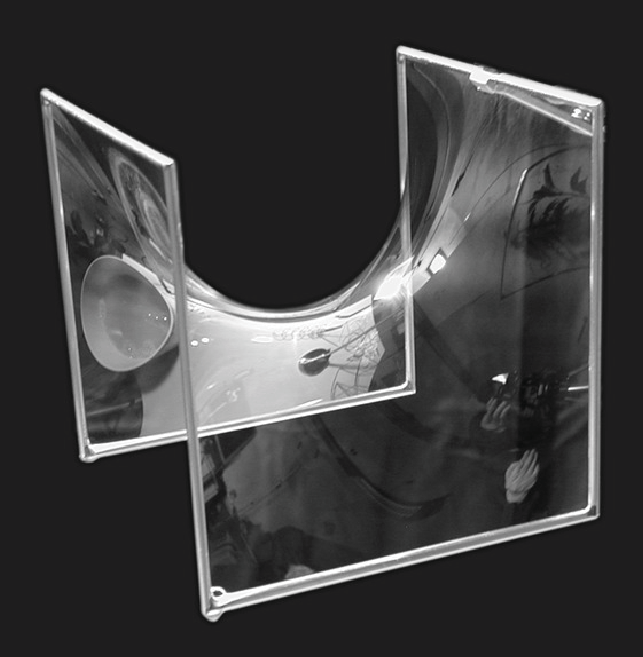
\includegraphics[width=11em]{../Slike/Soap_Film.png}
    \end{minipage}
    \hfill 
    \begin{minipage}{0.45\linewidth}
        \centering
        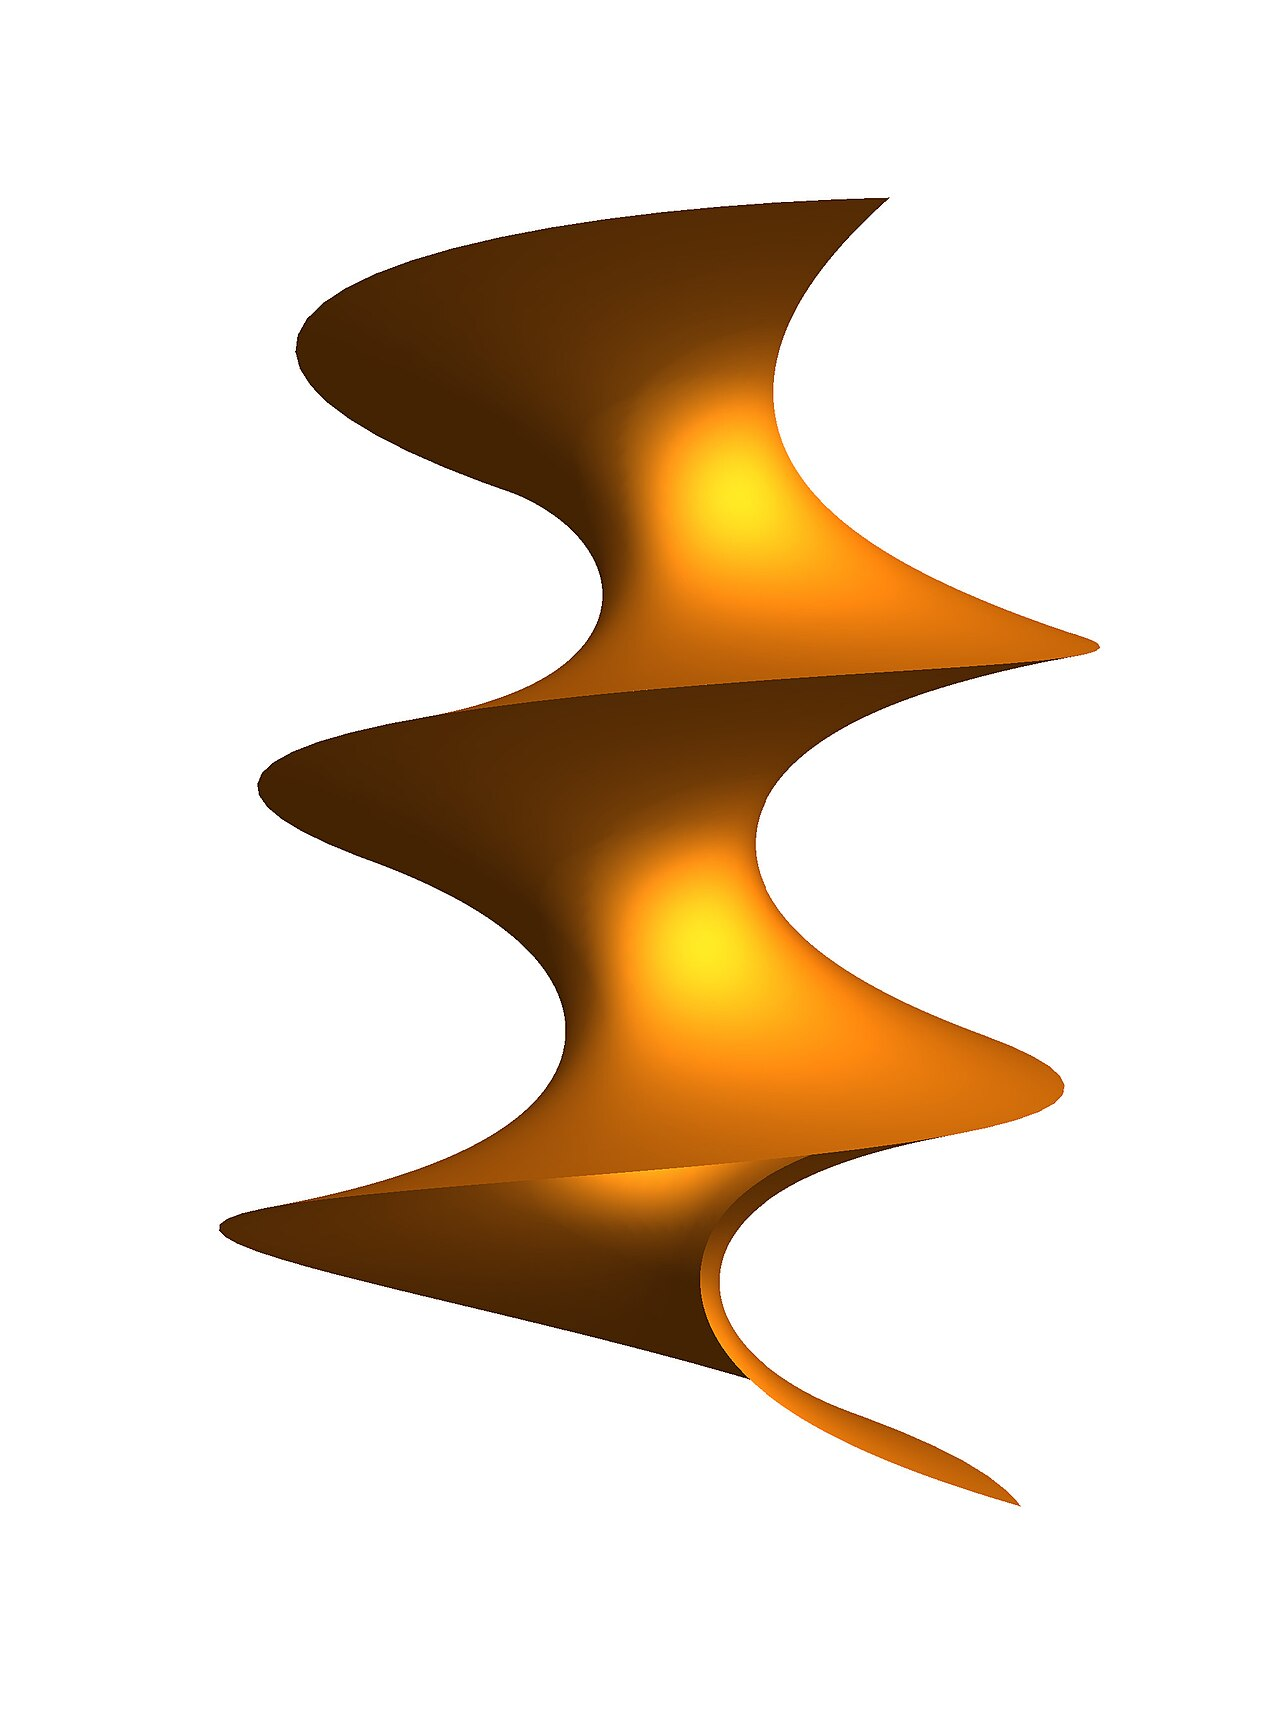
\includegraphics[width=11em]{../Slike/Helically_Rotated_Catenary.jpg}
    \end{minipage}

\end{frame}

\begin{frame}
    \frametitle{Srednja ukrivljenost}

    \begin{definicija}
        Naj bo $\gamma: t \mapsto(x(t), y(t))$ regularna $C^2$ parametrizacija krivulje. Potem polarni kot $\phi(t):=\arg (\dot{x}(t), \dot{y}(t))$ obstaja za vse $t$. \emph{Predznačeno ukrivljenost} definiramo kot: 
        $$
        \kappa:=\frac{d \phi}{d s}=\frac{\ddot{y} \dot{x}-\ddot{x} \dot{y}}{\left(\dot{x}^2+\dot{y}^2\right)^{3 / 2}}
        $$
    \end{definicija}

    Naj bo $S$ ploskev v $\mathbb{R}^3$ in $p$ točka na $S$. Vsaka ravnina skozi $p$, ki vsebuje normalo na ploskev na $S$ odreže krivuljo. Ko to ravnino vrtimo za kot $\theta$, se ukrivljenost krivulje spreminja. 

    \begin{definicija}
        Za točko $p \in S$ definiramo srednjo ukrivljenost kot: 
        $$
        H=\frac{1}{2 \pi} \int_0^{2 \pi} \kappa(\theta) \, d \theta
        $$
    \end{definicija}
\end{frame}

\begin{frame}
    \frametitle{Srednja ukrivljenost}

    Alternativne karakterizacije srednje ukrivljenosti:
    \begin{itemize}
        \item[$\bullet$] $H=\frac{1}{2}\left(\kappa_1+\kappa_2\right)$, kjer sta $\kappa_1$ in $\kappa_2$ glavni ukrivljenosti; 
        \item[$\bullet$] $2 H=\operatorname{sl}\left((\mathrm{II})\left(\mathrm{I}^{-1}\right)\right)$, kjer sta $\mathrm{I}$ in $\mathrm{II}$ prva in druga fundamentalna forma.
    \end{itemize}

    \begin{trditev}
        Minimalne ploskve so tiste, ki imajo srednjo ukrivljenost $0$, t.j. $H=0$. 
    \end{trditev}
    
    \vspace{1em}
    Naj bo $r=r(u, v)$ regularna parametrizacija ploskve $S$. 
   
    \begin{definicija}
        Prvo fundamentalno formo definiramo kot: 
        $$
        \mathrm{I}=E d u^2+2 F d u d v+G d v^2
        $$
        Koeficienti $E, F$ in $G$ so definirani kot: 
        $$
        E(u, v)=r_u \cdot r_u, \quad F(u, v)=r_u \cdot r_v, \quad G(u, v)=r_v \cdot r_v
        $$
    \end{definicija}
\end{frame}

\begin{frame}
    \frametitle{Srednja ukrivljenost}

    \begin{definicija}
        Drugo fundamentalno formo definiramo kot:
        $$
        \mathrm{II}=L d u^2+2 M d u d v+N d v^2
        $$
        Koeficiente $L, M$ in $N$ dobimo kot projekcije drugih parcialnih odvodov $r$ na enostki normalni vektor $n=\frac{r_u \times r_v}{\left|r_u \times r_v\right|}$. Torej: 
        $$
        L=\langle r_{u u}, n \rangle, \quad M=\langle r_{u v}, n\rangle, \quad N= \langle r_{v v}, n \rangle
        $$
        
    \end{definicija}

    Matrika prve fundamentalne forme je $\begin{bmatrix} E & F \\ F & G \end{bmatrix}$.
    
    Matrika druge fundamentalne forme v bazi $\{r_u, r_v\}$ je $\begin{bmatrix} L & M \\ M & N \end{bmatrix}$.

    Srednjo ukrivljenost lahko tako izrazimo kot: 
    $$
    H=\frac{1}{2} \frac{E N-2 F M+G L}{E G-F^2}
    $$
\end{frame}

\begin{frame}
    \frametitle{Weierstrass-Enneperjeva parametrizacija}

    \begin{izrek}
        Naj bosta $f$ in $g$ funkciji enotskem disku ali kompleksni ravnini taki, da je $f$ holomorfna, $g$ meromorfna in $f g^2$ holomorfna. Naj bodo $c_1, c_2, c_3$ kompleksne konstante. Potem je ploskev, podana s spodnjo parametrizacijo minimalna:
        $$
        \begin{aligned}
            r_k(\zeta) & =\operatorname{Re}\left\{\int_0^\zeta \varphi_k(z) \, dz\right\}+c_k, \quad k=1,2,3 \\
            \varphi_1 & =f\left(1-g^2\right) / 2 \\
            \varphi_2 & =i f\left(1+g^2\right) / 2 \\
            \varphi_3 & =f g
        \end{aligned}
        $$
        Še več, vsaka minimalna ploskev, ki ima parametrizacijo, se da lokalno predstaviti na tak način.
    \end{izrek}
\end{frame}

\end{document}